\exercise{8|1}{Grundlagen der Organisation}

Nennen Sie Gründe und Anlässe, die dazu führen, dass in einem Unternehmen organisiert wird.

\solution{
\textbf{Gründe für die Organisation in Unternehmen:}
\begin{itemize}
    \item Arbeitsteilung
    \item verschiedene Aufgabenarten
    \item hohe Anzahl an Mitarbeitern
\end{itemize}

\textbf{Notwendigkeit zur Organisation:}  
In einem Unternehmen entsteht die Notwendigkeit zur Organisation immer dann, wenn sich die für die formale Organisationsstruktur relevanten Entscheidungsstabstellen und Einflussfaktoren verändert haben.

\textbf{Einflussfaktoren:}  
Diese können in unternehmensinterne und unternehmensexterne Faktoren unterteilt werden:

\begin{itemize}
    \item \textbf{Unternehmensinterne Faktoren, wie z. B.:}
    \begin{itemize}
        \item Wachstum (Eintritt in neue Märkte, Erweiterung des bestehenden Leistungsprogramms, Diversifikation)
        \item Straffung des Leistungsprogramms
        \item Kooperationen
        \item neue EDV-Systeme
        \item neue Technologien
        \item Kosten- und Synergieüberlegungen (z. B. Zusammenlegung von Standorten)
    \end{itemize}
    \item \textbf{Unternehmensexterne Faktoren, wie z. B.:}
    \begin{itemize}
        \item rechtliche Regelungen (z. B. in den Bereichen Arbeits- und Wirtschaftsrecht)
        \item Einfluss der Anspruchsgruppen (z. B. ökologische Aspekte)
        \item wirtschaftliche Lage (z. B. Rezession)
    \end{itemize}
\end{itemize}
}

\exercise{8|2}{Aufbau- und Ablauforganisation}

Jedes Unternehmen steht vor dem Problem, Strukturen und Prozesse festzulegen. Dazu dienen die Aufbau- und Ablauforganisation.

\begin{enumerate}[label=\alph*)]
    \item Zeigen Sie allgemein die Zusammenhänge zwischen der Aufbau- und der Ablauforganisation.
    \item Beschreiben Sie an einem selbst gewählten Beispiel die Zusammenhänge zwischen der Aufbau- und der Ablauforganisation.
\end{enumerate}

\solution{
\begin{enumerate}[label=\alph*)]
    \item \textbf{Allgemeine Zusammenhänge zwischen Aufbau- und Ablauforganisation:}
    \begin{itemize}
        \item Aufbau- und Ablauforganisation hängen sehr eng zusammen.
        \item Beide betrachten das gleiche Objekt, wenn auch unter verschiedenen Aspekten.
        \item Sie bedingen sich gegenseitig und bauen aufeinander auf.
        \item Die Aufbauorganisation liefert den organisatorischen Rahmen, innerhalb dessen die erforderlichen Prozesse der Ablauforganisation vollziehen.
        \item Ausgangspunkt der Ablauforganisation stellen die durch die Aufgabenanalyse gewonnenen Elementaraufgaben dar.
        \item Die Arbeitsanalyse und -synthese als Aspekte der Ablauforganisation bauen auf den Ergebnissen der Aufgabenanalyse auf.
        \item Als erster Schritt steht die Aufgabenanalyse, welche die Gesamtaufgabe in einzelne Elementaraufgaben gliedert.
        \item Darauf aufbauend werden aus einem mithilfe der Aufgabenanalyse gewonnenen Aufgabenkomplex gebildete Einheiten (z. B. Abteilungen oder anderen Aufgabenträgern) zugeordnet (Aufbauorganisation).
        \item Zur Ausführung kommen die in der Arbeitsanalyse auf die Elementaraufgaben zerlegten Aufgaben in Form der Ablauforganisation, d. h. Tätigkeiten zur Erfüllung einer Aufgabe werden unter Berücksichtigung des Arbeitsablaufs, der Arbeitszeit und der Arbeitsmittel zusammengefasst.
    \end{itemize}

    \item \textbf{Beispiel für die Zusammenhänge:}\\
    (Hier kann ein beliebiges Beispiel eingefügt werden, das die Zusammenhänge zwischen Aufbau- und Ablauforganisation verdeutlicht, z. B. die Organisation eines Produktionsprozesses in einem Unternehmen.)
\end{enumerate}
}

\exercise{8|3}{Formale vs. informale Organisation}
In jeder Organisation existieren neben der bewusst gestalteten formalen Organisationsstruktur auch informale Strukturen.

\begin{enumerate}[label=\alph*)]
    \item Wie erkennen Sie formale und informale Organisationsstrukturen? Geben Sie Beispiele für informale Organisationssituationen.
    \item Welche Bedeutung hat die informale Organisation in Bezug auf die Erreichung der Unternehmensziele?
\end{enumerate}

\solution{
\begin{enumerate}[label=\alph*)]
    \item 
    \textbf{Formale Organisationsstruktur:}
    \begin{itemize}
        \item Bei der formalen Struktur handelt es sich um die bewusst gestaltete Organisation.
        \item Hier werden die Abläufe und der Aufbau (Stellenbildung) beschrieben.
    \end{itemize}
    \textbf{Informale Organisationsstruktur:}
    \begin{itemize}
        \item Informale Strukturen bilden sich aus der betrieblichen Wirklichkeit heraus und treten neben oder anstelle der formalen Organisation.
        \item Als Ursache dieser Erscheinung können menschliche Eigenheiten (z. B. Sympathie, gemeinsame Interessen), der soziale Status der Mitglieder des Unternehmens (z. B. Management- vs. Facharbeiterebene), die Arbeitsbedingungen (z. B. Zeitdruck) oder die zu lösende Aufgabe (z. B. ein spezielles Projekt) genannt werden.
        \item Über die informale Organisation gibt es zumeist keine Dokumentation, da sie schwieriger zu erfassen und zu dokumentieren ist als die formale.
        \item Manchmal ist sie auch Ausdruck von Unzufriedenheit der Mitarbeitenden gegenüber der formalen Organisation, respektive von mangelnder Praktikabilität in der betrieblichen Realität.
    \end{itemize}
    
    \item 
    \textbf{Bedeutung der informalen Organisation:}
    \begin{itemize}
        \item Über die Auswirkungen der informalen Struktur kann keine allgemeingültige Aussage gemacht werden.
        \item Eine informale Struktur kann die Kommunikation und somit die Zusammenarbeit der Mitarbeitenden fördern, was sich wiederum positiv auf die Erreichung der Unternehmensziele auswirkt.
        \item Sie kann aber auch negative Auswirkungen in Form von ineffizienten Abläufen haben.
        \item Wichtig ist in jedem Fall, sich der informalen Struktur bewusst zu werden, um positive Wirkungen zu fördern und Konflikte zu beseitigen.
    \end{itemize}
\end{enumerate}
}

\exercise{8|4}{Dilemma der Ablaufplanung}
Erläutern Sie das Dilemma der Ablaufplanung.  
In welchen Unternehmen spielt diese Problematik eine besonders große Rolle?

\solution{
\begin{itemize}
    \item Bei der Ablaufplanung sind folgende Grundsätze einzuhalten:
    \begin{itemize}
        \item Prinzip der Termineinhaltung
        \item Prinzip der Zeitminimierung
        \item Prinzip der Kapazitätsauslastung
    \end{itemize}
    \item Die letzten beiden Grundsätze lassen sich nur selten gleichzeitig verwirklichen.
    \item Gutenberg spricht in diesem Fall vom Dilemma der Ablaufplanung.
    \item Das eigentliche Ziel der Ablauforganisation besteht somit in der optimalen Abstimmung dieser beiden Forderungen.
    \item Es geht darum, die Durchlaufzeit des Materials und die Leerzeiten von Maschinen und Menschen gleichzeitig zu minimieren.
    \item Dieses Dilemma spielt vor allem in großen Unternehmen mit Fließbandproduktion eine große Rolle.
    \item Durch die Digitalisierung gelingt es Unternehmen heute immer besser, mit dem Dilemma der Ablaufplanung umzugehen.
    \item Durch den Einsatz Künstlicher Intelligenz und die digitale Vernetzung der Wertschöpfungsprozesse (z. B. durch Internet of Things) gelingt es, Zeitminimierung und Kapazitätsauslastung optimal aufeinander abzustimmen.
\end{itemize}
}

\exercise{8|5}{Organisationsformen in der Praxis}
Beschreiben Sie, um welche Formen der Aufbauorganisation es sich in den folgenden Fällen jeweils handelt. Begründen Sie Ihre Entscheidung.

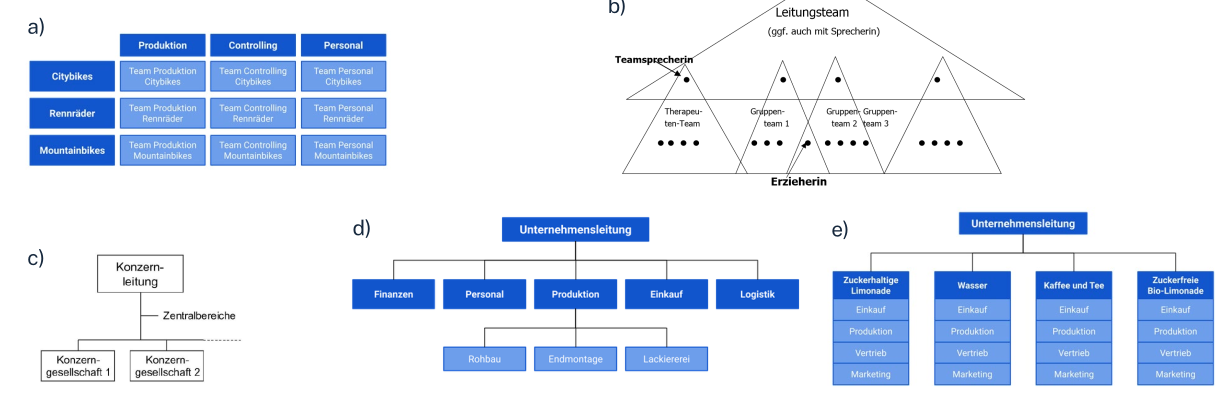
\includegraphics[width=\textwidth]{figures/8_5.png}

\solution{
\begin{itemize}
    \item \textbf{a) Matrixorganisation:} \\
    Beschreibung und Begründung der Entscheidung für die Matrixorganisation.
    \item \textbf{b) Teamorganisation eines Kindergartens:} \\
    Beschreibung und Begründung der Entscheidung für die Teamorganisation.
    \item \textbf{c) Holding:} \\
    Beschreibung und Begründung der Entscheidung für die Holding-Struktur.
    \item \textbf{d) Funktionale Organisation:} \\
    Beschreibung und Begründung der Entscheidung für die Funktionale Organisation.
    \item \textbf{e) Spartenorganisation:} \\
    Beschreibung und Begründung der Entscheidung für die Spartenorganisation.
\end{itemize}
}

